\chapter{Totaalsynthese: strategie en klassieke routes}\label{ch:b3:total-synthesis}

Het antikankermiddel paclitaxel werd eerst geïsoleerd uit de schors van
de westelijke taxus, een traag groeiende boom; het afstropen van de
schors doodde de boom, en de voorraad bleef ver achter bij wat patiënten
nodig hadden. Chemici antwoordden op twee manieren: met \omterm{def:b3:total-synthesis:total}{totaalsyntheses},
die aantoonden dat het molecuul uit eenvoudige uitgangsstoffen gebouwd
kon worden maar veel te lang waren voor de productie, en met een
\omterm{def:b3:total-synthesis:total}{semisynthese} uit een verwante verbinding die uit de naalden van een
gewone taxus gewonnen wordt, een hernieuwbare bron.
Dit hoofdstuk gaat over hoe zulke routes beoordeeld en ontworpen worden:
hoe rendementen zich vermenigvuldigen, waarom convergentie loont, wat
beschermende groepen kosten, welke bindingen eerst gevormd moeten worden,
en drie mijlpaalsyntheses, gelezen met die instrumenten.

\begin{recall}
Het deel van jaar~2 behandelde de retrosynthetische analyse
(doelmolecuul, disconnectie, synthon, synthetisch equivalent,
functionele-groepsinterconversie), orthogonale beschermende groepen, de
aldolreactie, de robinsonannulatie, de wittigreactie en de chemie van
iminiumionen; het deel van jaar~1 beschermende groepen en rendementen.
\Cref{ch:b3:asymmetric-synthesis},
\cref{ch:b3:pericyclic} en \cref{ch:b3:homogeneous-catalysis} leverden de
moderne sleutelstappen.
\end{recall}

\begin{omfigure}
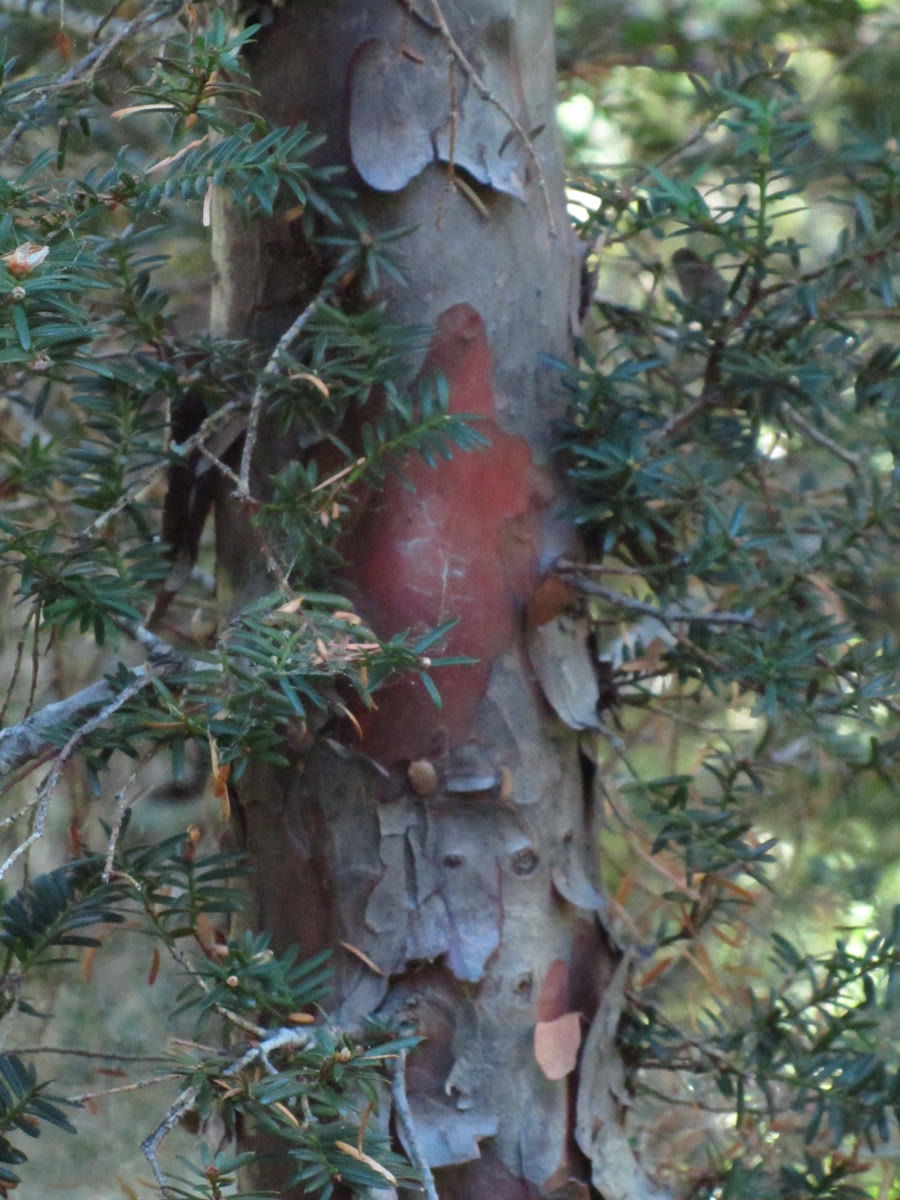
\includegraphics[width=0.32\linewidth]{images/book4/pacific-yew.jpg}

{\small Schors en naalden van een westelijke taxus, de eerste bron van
paclitaxel. Foto: JOE BLOWE, CC BY-SA 2.0.}
\end{omfigure}

\section{Een synthese meten}

\begin{definition}[Totaalsynthese]\label{def:b3:total-synthesis:total}
Een \emph{totaalsynthese}\index{totaalsynthese} maakt een complex
molecuul, vaak een natuurstof, uit eenvoudige commerciële verbindingen.
Een \emph{formele synthese}\index{formele synthese} maakt een
intermediair van een eerdere totaalsynthese, wat de route op papier
voltooit. Een \emph{semisynthese}\index{semisynthese} vertrekt van een
natuurlijke verbinding die al dicht bij het doelmolecuul ligt.
\end{definition}

\begin{definition}[Opbouw van een route]\label{def:b3:total-synthesis:architecture}
Bij een \emph{lineaire synthese}\index{lineaire synthese} werkt elke stap
in op het product van de vorige; bij een
\emph{convergente synthese}\index{convergente synthese} worden
afzonderlijke fragmenten parallel gemaakt en laat samengevoegd. De
\emph{langste lineaire reeks}\index{langste lineaire reeks} (LLS) is het
grootste aantal stappen van een uitgangsstof tot het doelmolecuul. Het
\emph{totaalrendement}\index{totaalrendement} is de verkregen hoeveelheid
doelmolecuul gedeeld door de hoeveelheid van de beperkende uitgangsstof.
\end{definition}

\begin{proposition}[Totaalrendement]\label{prop:b3:total-synthesis:overall-yield}
Voor een reeks stappen met rendementen $y_1, \dots, y_n$ is het \omterm{def:b3:total-synthesis:architecture}{totaalrendement} $Y = \prod_i y_i$.
\end{proposition}

\begin{proof}
Elke stap zet de hoeveelheid die hij ontvangt om in $y_i$ maal zoveel
product; de hoeveelheid die het doelmolecuul bereikt, is de
uitgangshoeveelheid, achtereenvolgens met elke factor vermenigvuldigd.
\end{proof}

\begin{proposition}[Convergentie]\label{prop:b3:total-synthesis:convergent}
Een route van $n = 2m + 1$ stappen met gelijk rendement $y$, opgebouwd als twee takken van $m$ stappen die door
één koppelingsstap samengevoegd worden, heeft langs haar \omterm{def:b3:total-synthesis:architecture}{langste
lineaire reeks} het \omterm{def:b3:total-synthesis:architecture}{totaalrendement} $y^{m+1}$,
tegenover $y^{2m+1}$ voor de lineaire route met dezelfde stappen.
\end{proposition}

\begin{proof}
Elke tak wordt afzonderlijk gemaakt, met zoveel uitgangsstof als nodig:
het materiaal van elke tak doorloopt $m$ stappen en daarna de koppeling, $m + 1$
factoren $y$. Bij de lineaire route doorloopt het materiaal alle $2m + 1$. Voor $m = 10$
en $y = 0.90$: 31\,\% tegenover 11\,\%.
\end{proof}

\begin{omfigure}
\begin{tikzpicture}
\begin{axis}[width=0.7\linewidth, height=5.8cm, xmin=0, xmax=30, ymin=0, ymax=1.02,
  axis lines=left, xlabel={aantal stappen $n$}, ylabel={totaalrendement},
  tick label style={font=\scriptsize}, label style={font=\small},
  legend style={font=\scriptsize, draw=none, at={(1.03,0.5)}, anchor=west}, legend cell align=left]
\addplot[color=omDef, thick] table[x=n, y=y95] {figdata/out/bachelor-3-overall-yield.dat};
\addlegendentry{95\,\% per stap}
\addplot[color=omMeth, thick] table[x=n, y=y90] {figdata/out/bachelor-3-overall-yield.dat};
\addlegendentry{90\,\%}
\addplot[color=omThm, thick] table[x=n, y=y80] {figdata/out/bachelor-3-overall-yield.dat};
\addlegendentry{80\,\%}
\addplot[color=omMeth, thick, dashed, mark=*, mark size=1pt] table[x=n, y=y90] {figdata/out/bachelor-3-overall-yield-b.dat};
\addlegendentry{90\,\%, convergent}
\end{axis}
\end{tikzpicture}

{\small \omterm{def:b3:total-synthesis:architecture}{Totaalrendement} tegen het aantal stappen voor drie rendementen per
stap (volle lijnen: lineaire routes), en voor convergente routes bij
90\,\% per stap (twee gelijke takken die in een laatste stap samengevoegd
worden; gestreept). Twintig stappen bij 90\,\% laten 12\,\% over;
dezelfde stappen convergent geschikt laten ongeveer drie keer meer over.}
\end{omfigure}

\begin{omfigure}
\begin{tikzpicture}[font=\scriptsize, >=Stealth, node distance=0.9cm,
  st/.style={circle, draw, fill=omDef!15, minimum size=4mm, inner sep=0pt}]
  \foreach \i in {0,...,6} { \node[st] (l\i) at (\i*0.9,1.6) {}; }
  \foreach \i in {0,...,5} { \pgfmathtruncatemacro\j{\i+1} \draw[->] (l\i) -- (l\j); }
  \node[anchor=west] at (6.0,1.6) {lineair: 6 stappen, LLS 6};
  \foreach \i in {0,...,2} { \node[st] (a\i) at (\i*0.9,0.6) {}; \node[st] (b\i) at (\i*0.9,-0.6) {}; }
  \draw[->] (a0) -- (a1); \draw[->] (a1) -- (a2); \draw[->] (b0) -- (b1); \draw[->] (b1) -- (b2);
  \node[st, fill=omThm!25] (t) at (3.0,0) {};
  \draw[->] (a2) -- (t); \draw[->] (b2) -- (t);
  \node[anchor=west] at (3.4,0) {convergent: 5 stappen, LLS 3};
\end{tikzpicture}

{\small Routebomen: elke cirkel is een verbinding, elke pijl een stap. Een
lineaire route stuurt al haar materiaal door elke stap; een convergente
route maakt twee fragmenten naast elkaar en koppelt ze, zodat haar
\omterm{def:b3:total-synthesis:architecture}{langste lineaire reeks} korter is.}
\end{omfigure}

\begin{definition}[Economieën en idealiteit]\label{def:b3:total-synthesis:economy}
\emph{Stapeconomie}\index{stapeconomie} is het streven een doelmolecuul in
zo weinig mogelijk stappen te bereiken;
\emph{beschermgroepeconomie}\index{beschermgroepeconomie}, het streven zo
weinig mogelijk beschermings- en ontschermingsstappen te gebruiken. De
\emph{idealiteit}\index{idealiteit} van een route is de fractie van haar
stappen die het skelet opbouwen of een noodzakelijke verandering van
oxidatieniveau uitvoeren:
$(\text{opbouwstappen} + \text{strategische redoxstappen})/(\text{totaal aantal stappen})$.
\end{definition}

\begin{proposition}[Idealiteit van een route]\label{prop:b3:total-synthesis:ideality}
Een eenpotsroute die alleen skeletbindingen vormt, heeft een \omterm{def:b3:total-synthesis:economy}{idealiteit}
van 100\,\%; elke bescherming, ontscherming,
functionele-groepsinterconversie of niet-strategische redoxstap
verlaagt haar.
\end{proposition}

\begin{proof}
Rechtstreeks uit de definitie: zulke stappen vergroten de noemer zonder
de teller te vergroten.
\end{proof}

\section{Beschermende groepen en hun economie}

Elke beschermende groep kost minstens twee stappen, de reagentia om haar
aan te brengen en te verwijderen, en het materiaal dat bij beide verloren
gaat. Een route van acht stappen bij 90\,\% behoudt 43\,\% van haar
materiaal; twee beschermingen en twee ontschermingen bij elk 95\,\%
toevoegen brengt dat op 35\,\%. Beschermende groepen worden orthogonaal
gekozen, zodat elke groep verwijderd kan worden zonder de andere aan te
tasten; beter nog wordt de volgorde van de stappen zo geschikt dat de
reactieve groep niet aanwezig is, of nog niet vrijgemaakt, wanneer ze
zou storen: syntheses zonder beschermende groepen zijn een doel, geen
curiositeit.

\begin{method}[Een totaalsynthese lezen]\label{met:b3:total-synthesis:analyse}
\begin{enumerate}
  \item Bepaal de ringen, stereocentra en gevoelige groepen van het
        doelmolecuul.
  \item Zoek de belangrijkste disconnecties en de reacties die ze in de
        voorwaartse richting tot stand brengen (\omterm{def:b3:total-synthesis:strategic-bond}{strategische bindingen}).
  \item Tel de stappen en zoek de \omterm{def:b3:total-synthesis:architecture}{langste lineaire reeks}; noteer de
        convergentie.
  \item Noteer hoe elk stereocentrum vastgelegd wordt (substraatcontrole,
        hulpgroep, katalysator, \omterm{def:b3:asymmetric-synthesis:chiral-pool}{chirale pool}).
  \item Som de beschermende groepen en de andere niet-ideale stappen op;
        bereken het \omterm{def:b3:total-synthesis:architecture}{totaalrendement} en de \omterm{def:b3:total-synthesis:economy}{idealiteit}.
\end{enumerate}
\end{method}

\begin{method}[Stappen tellen]\label{met:b3:total-synthesis:count}
\begin{enumerate}
  \item Een stap is één bewerking die eindigt met een geïsoleerd (of
        minstens opgewerkt) product; een eenpotsreeks zonder isolatie telt
        als één stap.
  \item Tel alle stappen voor het totaal; volg voor de LLS de langste weg
        van een commerciële verbinding naar het doelmolecuul.
  \item Vermenigvuldig de rendementen langs de LLS voor het
        \omterm{def:b3:total-synthesis:architecture}{totaalrendement}.
\end{enumerate}
\end{method}

\section{Strategische bindingen en sleutelstappen die ringen vormen}

\begin{definition}[Strategische binding]\label{def:b3:total-synthesis:strategic-bond}
Een \emph{strategische binding} van een doelmolecuul\index{strategische binding}
is een binding waarvan de disconnectie het doelmolecuul het sterkst
vereenvoudigt, meestal door een ringsysteem te splitsen of meerdere
stereocentra tegelijk weg te nemen, en die een betrouwbare reactie kan
vormen.
\end{definition}

Ringvormende reacties die twee bindingen of meerdere stereocentra
tegelijk maken, zijn de werkpaarden: de diels-alderreactie (twee
bindingen C--C, tot vier stereocentra, stereospecifiek,
\cref{ch:b3:pericyclic}), de robinsonannulatie (een zesring op een
keton), \omterm{def:b3:homogeneous-catalysis:metathesis}{ringsluitende metathese}
(\cref{ch:b3:homogeneous-catalysis}) voor middelgrote en grote ringen, en
cascades.

\begin{definition}[Cascadereactie]\label{def:b3:total-synthesis:cascade}
Een \emph{cascadereactie}\index{cascadereactie} is een reeks omzettingen
waarin elke stap de functionaliteit voor de volgende maakt, zonder
intermediairen te isoleren of reagentia toe te voegen.
\end{definition}

\begin{definition}[Biomimetische synthese]\label{def:b3:total-synthesis:biomimetic}
Een \emph{biomimetische synthese}\index{biomimetische synthese} bootst de
route na waarlangs een natuurstof vermoedelijk in het organisme gemaakt
wordt.
\end{definition}

De cyclisatie van squaleenoxide tot lanosterol in cellen, vier ringen en
zeven stereocentra in één enzymatische cascade, inspireerde de
polyeencyclisaties van William Johnson, waarin een kation dat aan één
uiteinde van een zorgvuldig ontworpen polyeen ontstaat, ring na ring
sluit via stoelvormige overgangstoestanden, en daarbij de
\textit{trans}-ringverbindingen van de steroïden vastlegt.

\section{Mijlpaalroutes}

\begin{definition}[Mannichreactie]\label{def:b3:total-synthesis:mannich}
De \emph{mannichreactie}\index{mannichreactie} is de additie van een enol
of enolaat aan een iminiumion, in situ gemaakt uit een aldehyde en een
primair of secundair amine, wat een $\beta$-aminocarbonylverbinding geeft.
\end{definition}

In 1917 maakte Robert Robinson tropinon, het bicyclische hart van
atropine en cocaïne, in één pot uit drie eenvoudige componenten in water,
in de veronderstelling dat de plant het misschien op dezelfde manier
opbouwt:
$\ce{C4H6O2 + CH3NH2 + C5H6O5 -> C8H13NO + 2CO2 + 2H2O}$ (succinaldehyde, methylamine en
acetondicarbonzuur geven tropinon).

\begin{omfigure}
\begin{tikzpicture}[font=\small, >=Stealth]
  \node[align=center] at (-0.5,0) {$\ce{OHC-CH2CH2-CHO}$\\ $+\ \ce{CH3NH2}$\\ $+\ \ce{HO2C-CH2-CO-CH2-CO2H}$};
  \draw[->, thick] (3.0,0) -- (4.7,0) node[midway, above, font=\scriptsize] {gebufferd water} node[midway, below, font=\scriptsize] {$-\ce{2CO2}$, $-\ce{2H2O}$};
  \begin{scope}[xshift=6.1cm, yshift=-0.2cm]
    \coordinate (c1) at (-1,0.3); \coordinate (c2) at (-0.8,-0.5); \coordinate (c3) at (0,-0.9);
    \coordinate (c4) at (0.8,-0.5); \coordinate (c5) at (1,0.3); \coordinate (c6) at (0.45,1.15);
    \coordinate (c7) at (-0.45,1.15); \coordinate (n) at (0,0.45);
    \draw[thick] (c1) -- (c2) -- (c3) -- (c4) -- (c5) -- (c6);
    \draw[thick] (c7) -- (c1);
    \draw[thick] (c6) -- (0.12,1.15); \draw[thick] (-0.12,1.15) -- (c7);
    \draw[thick] (c1) -- (n) -- (c5);
    \draw[thick] (n) -- (0,1.6) node[above, inner sep=1pt] {$\ce{CH3}$};
    \draw[thick, double, double distance=1.5pt] (c3) -- (0,-1.55) node[below, inner sep=1pt] {O};
    \node[fill=white, inner sep=0.5pt] at (n) {N};
    \node[font=\scriptsize, anchor=west] at (1.2,0.3) {tropinon};
  \end{scope}
\end{tikzpicture}

{\small De tropinonsynthese van Robinson. Twee \omterm{def:b3:total-synthesis:mannich}{mannichreacties}, de eerste
intermoleculair en de tweede ringsluitend, verbinden de drie componenten;
de twee carbonzuurgroepen die de centrale groepen $\ce{CH2}$ enoliseerbaar maakten, vertrekken
daarna als koolstofdioxide. In het bicyclische product overspant de
N-methylbrug de zevenring.}
\end{omfigure}

\begin{proposition}[Tropinon in één pot]\label{prop:b3:total-synthesis:tropinone}
De eenpotssynthese van tropinon bestaat uit twee \omterm{def:b3:total-synthesis:mannich}{mannichreacties} gevolgd
door twee decarboxyleringen.
\end{proposition}

\begin{proof}[Beargumenteerd]
Methylamine en één aldehydegroep van succinaldehyde geven een
iminiumion; een enol van acetondicarbonzuur addeert eraan (eerste
\omterm{def:b3:total-synthesis:mannich}{mannichreactie}). Het gevormde secundaire amine condenseert met de tweede
aldehydegroep tot een cyclisch iminiumion, dat door het enol aan de
andere kant van het keton aangevallen wordt (tweede \omterm{def:b3:total-synthesis:mannich}{mannichreactie}),
wat de bicyclus sluit. De twee $\beta$-ketozuurgroepen verliezen daarna $\ce{CO2}$, zoals $\beta$-ketozuren doen
bij zacht verwarmen.
\end{proof}

De synthese van prostaglandine $\mathrm F_{2\alpha}$ door Elias Corey (1969) maakte de
retrosynthetische analyse expliciet. Een bicyclo[2.2.1]heptenon,
gebouwd met een diels-alderreactie, draagt de relatieve configuratie van
de substituenten van het cyclopentaan; een
\omterm{def:b3:radicals-carbenes:baeyer}{baeyer-villigeroxidatie} (\cref{ch:b3:radicals-carbenes}) en een
jodolactonisatie zetten het om in het coreylacton, waaraan de twee
zijketens via olefineringen gekoppeld worden. Het lacton heeft sindsdien
voor veel prostaglandinegeneesmiddelen gediend.

\begin{omfigure}
\begin{tikzpicture}[font=\small,
  box/.style={draw, rounded corners, align=center, fill=omDef!8, inner sep=4pt}]
  \node[box] (t) at (0,0) {prostaglandine\\ $\mathrm F_{2\alpha}$};
  \node[box] (l) at (4.4,0) {coreylacton\\ (vier\\ stereocentra)};
  \node[box] (b) at (9.2,0) {bicyclo[2.2.1]-\\ heptenon};
  \node[box] (d) at (9.2,-2.4) {gesubstitueerd\\ cyclopentadieen $+$\\ keteenequivalent};
  \draw[omretro] (t) -- (l) node[midway, above=3pt, font=\scriptsize] {olefineringen};
  \draw[omretro] (l) -- (b) node[midway, above=3pt, font=\scriptsize, align=center] {jodolactonisatie,\\ Baeyer-Villiger};
  \draw[omretro] (b) -- (d) node[midway, right, font=\scriptsize] {Diels-Alder};
\end{tikzpicture}

{\small De retrosynthese van prostaglandine $\mathrm F_{2\alpha}$ door Corey, in grote lijnen (dubbele pijlen: ``wordt
gemaakt uit''). De twee zijketens worden eerst gedisconnecteerd; het
cyclopentaan met zijn vier stereocentra komt uit een lacton, het lacton
uit een bicyclisch keton, en het keton uit een diels-alderreactie die hun
relatieve configuratie vastlegt.}
\end{omfigure}

Oseltamivir, het griepmiddel, wordt industrieel gemaakt uit shikimizuur,
een verbinding uit de \omterm{def:b3:asymmetric-synthesis:chiral-pool}{chirale pool} die uit steranijs gewonnen en later
door fermentatie geproduceerd werd: zijn zesring en stereocentra zijn al
aanwezig. De route zet het ringdiol om in een epoxide, opent dat met
azide, sluit een aziridine en opent dat opnieuw met azide, waarbij de
twee stikstofatomen \textit{trans} komen te staan; acetylering en reductie
voltooien het werk. Omdat natriumazide en organische aziden giftig en op
grote schaal mogelijk explosief zijn, werden later routes zonder azide
ontwikkeld.

\begin{omfigure}
\begin{tikzpicture}[font=\scriptsize, >=Stealth,
  box/.style={draw, rounded corners, align=center, fill=omMeth!8, inner sep=3pt}]
  \node[box] (a) at (0,0) {($-$)-shikimizuur\\ (chirale pool)};
  \node[box] (b) at (3.1,0) {ester, ketal,\\ mesylaat};
  \node[box] (c) at (6.0,0) {epoxide};
  \node[box] (d) at (8.6,0) {azidoalcohol};
  \node[box] (e) at (8.6,-1.5) {aziridine};
  \node[box] (f) at (5.4,-1.5) {\textit{trans}-diamine-\\ precursor (azide)};
  \node[box] (g) at (1.6,-1.5) {oseltamivir-\\ fosfaat};
  \draw[->] (a) -- (b); \draw[->] (b) -- (c); \draw[->] (c) -- (d) node[midway, above] {$\ce{N3-}$};
  \draw[->] (d) -- (e); \draw[->] (e) -- (f) node[midway, above] {$\ce{N3-}$};
  \draw[->] (f) -- (g) node[midway, below, align=center] {acetylering,\\ reductie};
\end{tikzpicture}

{\small Oseltamivir uit shikimizuur, alleen de sleutelstadia: de
natuurlijke ring en zijn stereocentra blijven behouden, en twee
stikstofatomen worden \textit{trans} ten opzichte van elkaar ingevoerd
door de opeenvolgende opening van een epoxide en een aziridine met azide.}
\end{omfigure}

\section{Van ontdekking tot proces}

Een route die milligrammen levert voor biologische tests, is zelden
degene die voor tonnen gebruikt wordt. Proceschemici zoeken routes op
kosten, veiligheid en robuustheid: ze vervangen chromatografie door
kristallisatie, vervangen gevaarlijke reagentia en cryogene
temperaturen, verkorten de reeks, controleren met calorimetrie de
thermische veiligheid van elke stap, en leggen specificaties voor
onzuiverheden vast. Deze keuzes sluiten aan bij de maatstaven van
\cref{ch:b3:green-industrial}.

\begin{inthelab}[Van één gram naar één kilogram]
Een stap die op één gram in een rondbodemkolf uitgevoerd werd, wordt
herhaald op tien gram in een reactor met mantel, een bovenroerder en een
temperatuurvoeler in de vloeistof, waarbij het reactieve reagens met een
gecontroleerde snelheid toegevoegd wordt terwijl men de inwendige
temperatuur volgt: de vrijgezette warmte groeit met het volume, maar het
oppervlak dat haar afvoert groeit alleen met het kwadraat van de afmeting. Pas
als de warmtestroom en de opwerking (fasescheidingen, filtraties, drogen)
zich goed gedragen, wordt de stap op een kilogram uitgevoerd.
\end{inthelab}

\begin{safety}{\ghs[0.62cm]{GHS06}\ghs[0.62cm]{GHS08}\ghs[0.62cm]{GHS09}}
% ledger: ghs4:NaN3
Natriumazide: dodelijk bij inslikken, zeer giftig voor in het water
levende organismen; met zuren zet het waterstofazide vrij, een giftig en
explosief gas, en met zware metalen (koper en lood in afvoerleidingen)
vormt het explosieve aziden. Afval wordt chemisch vernietigd, nooit
weggegoten.
\end{safety}

\begin{history}[Robinson, Woodward, Corey]
Robert Robinson ontving de Nobelprijs voor de Scheikunde van 1947 voor
zijn werk over alkaloïden en andere plantaardige producten; zijn
tropinonsynthese van 1917 wordt nog steeds aangehaald om haar
zuinigheid. De syntheses van kinine, cholesterol, chlorofyl en, met
Albert Eschenmoser, vitamine $\mathrm B_{12}$ door Robert Woodward maakten van de
\omterm{def:b3:total-synthesis:total}{totaalsynthese} een kunst (prijs van 1965). Elias Corey formaliseerde de
retrosynthetische analyse en ontving de prijs van 1990 voor de theorie
en de methodologie van de organische synthese.
\end{history}

\section{Oefeningen}

\begin{exercise}[$\star$]\label{exo:b3:total-synthesis:1}
Bereken het \omterm{def:b3:total-synthesis:architecture}{totaalrendement} van lineaire routes van 10 en 20 stappen bij
90\,\% en bij 80\,\% per stap.
\end{exercise}

\begin{exercise}[$\star$]\label{exo:b3:total-synthesis:2}
Een route maakt fragment A in vijf stappen en fragment B in drie, koppelt
ze, en heeft nog vier stappen nodig tot het doelmolecuul. Geef het totale
aantal stappen en de \omterm{def:b3:total-synthesis:architecture}{langste lineaire reeks}.
\end{exercise}

\begin{exercise}[$\star$]\label{exo:b3:total-synthesis:3}
Geef het product van de \omterm{def:b3:total-synthesis:mannich}{mannichreactie} van aceton, formaldehyde en
dimethylamine.
\end{exercise}

\begin{exercise}[$\star$]\label{exo:b3:total-synthesis:4}
Geef een disconnectie volgens Diels-Alder van 4-acetylcyclohexeen, en de
voorwaartse reactie.
\end{exercise}

\begin{exercise}[$\star\star$]\label{exo:b3:total-synthesis:5}
Een lineaire route van 21 stappen verloopt met 90\,\% per stap. Bereken
haar \omterm{def:b3:total-synthesis:architecture}{totaalrendement} en dat van een convergente versie met twee takken
van 10 stappen en één koppeling.
\end{exercise}

\begin{exercise}[$\star\star$]\label{exo:b3:total-synthesis:6}
Route A heeft 12 stappen, waarvan 7 skeletbindingen vormen en 1 een
strategische reductie is; route B heeft 9 stappen, waarvan 7 skeletstappen.
Bereken hun \omterm{def:b3:total-synthesis:economy}{idealiteit}.
\end{exercise}

\begin{exercise}[$\star\star$]\label{exo:b3:total-synthesis:7}
Een route van acht stappen bij 90\,\% per stap heeft twee beschermende
groepen nodig, die elk met 95\,\% aangebracht en verwijderd worden.
Bereken het \omterm{def:b3:total-synthesis:architecture}{totaalrendement} met en zonder die groepen.
\end{exercise}

\begin{exercise}[$\star\star$]\label{exo:b3:total-synthesis:8}
Een triol heeft een primaire, een secundaire en een tertiaire
hydroxygroep. Stel beschermende groepen voor waarmee elke groep na elkaar
vrijgemaakt kan worden, en hun ontschermingsomstandigheden.
\end{exercise}

\begin{exercise}[$\star\star$]\label{exo:b3:total-synthesis:9}
Waarom werd paclitaxel geproduceerd door \omterm{def:b3:total-synthesis:total}{semisynthese} en niet via een van
zijn \omterm{def:b3:total-synthesis:total}{totaalsyntheses}?
\end{exercise}

\begin{exercise}[$\star\star\star$]\label{exo:b3:total-synthesis:10}
2-Methylcyclohexaan-1,3-dion reageert met methylvinylketon in een
robinsonannulatie. Duid de michael- en de aldolstap aan en geef het
gevormde bicyclische enon (het keton van Wieland-Miescher).
\end{exercise}

\begin{exercise}[$\star\star\star$]\label{exo:b3:total-synthesis:11}
Toon aan dat de convergente route van \cref{prop:b3:total-synthesis:convergent}
$y^{-m}$ keer meer materiaal behoudt dan de lineaire, en bereken deze factor voor $m = 5$ en
$m = 15$ bij 90\,\%.
\end{exercise}

\begin{exercise}[$\star\star\star$]\label{exo:b3:total-synthesis:12}
Waarom geven stoelvormige overgangstoestanden bij een
polyeencyclisatie \textit{trans}-ringverbindingen, en waarom is de geometrie (\textit{E} of \textit{Z}) van elke dubbele binding van belang?
\end{exercise}

\section{Probleem: tropinon in één pot}

\begin{problem}[{Weekendprobleem --- tropinon in één pot: de drie
componenten en de kloppende vergelijking, de twee mannichreacties, een
vergelijking met een lange lineaire route, en de stereochemie van
tropinon en zijn reductieproducten}]
\label{pb:b3:total-synthesis:1}
% ledger: aw:C, aw:H, aw:N, aw:O
Gegevens van het probleem: de eenpotssynthese, uitgevoerd in gebufferd
water rond pH 5, geeft tropinon met 42\,\% rendement; een oudere lineaire
route vereist 14 stappen met gemiddeld 75\,\%.

\medskip\noindent\textbf{Deel I --- Componenten en vergelijking.}
\begin{enumerate}
  \item Geef de formules van succinaldehyde, methylamine,
        acetondicarbonzuur en tropinon.
  \item Schrijf de kloppende vergelijking op.
  \item Bereken de molaire massa's van de beginstoffen en van tropinon.
  \item Bereken de atoomeconomie.
  \item Waarom gebruikt men acetondicarbonzuur in plaats van aceton?
  \item Waarom helpt een buffer rond neutrale pH?
\end{enumerate}

\medskip\noindent\textbf{Deel II --- Mechanisme.}
\begin{enumerate}[resume]
  \item Schrijf de vorming van het eerste iminiumion op.
  \item Toon de eerste \omterm{def:b3:total-synthesis:mannich}{mannichreactie}.
  \item Hoe ontstaat het tweede iminiumion?
  \item Toon de tweede, ringsluitende \omterm{def:b3:total-synthesis:mannich}{mannichreactie}.
  \item Waarom vertrekken de twee carbonzuurgroepen als $\ce{CO2}$?
  \item Tel de gevormde bindingen C--C en C--N.
\end{enumerate}

\medskip\noindent\textbf{Deel III --- Eén pot tegenover veertien stappen.}
\begin{enumerate}[resume]
  \item Bereken het \omterm{def:b3:total-synthesis:architecture}{totaalrendement} van de lineaire route.
  \item Bereken de verhouding van het eenpotsrendement daartoe.
  \item Bereken de \omterm{def:b3:total-synthesis:economy}{idealiteit} van de eenpotsroute.
  \item Wat pleit naast het rendement nog voor de eenpotsroute?
  \item Waarom noemt men de eenpotssynthese biomimetisch?
  \item Noem een andere reactieklasse uit dit hoofdstuk die meerdere
        bindingen tegelijk vormt.
\end{enumerate}

\medskip\noindent\textbf{Deel IV --- Stereochemie.}
\begin{enumerate}[resume]
  \item Is tropinon chiraal? Zoek zijn \omterm{def:b3:point-groups:operation}{symmetrie-element}.
  \item Waarom zijn de twee bruggenhoofdkoolstofatomen toch stereocentra?
  \item Reductie van het keton geeft twee alcoholen, tropine en
        pseudotropine. Wat is hun verband?
  \item Zijn tropine en pseudotropine chiraal?
  \item Waarom nadert een hydride de carbonylgroep bij voorkeur vanaf één
        vlak?
  \item Formuleer het resultaat: de verhouding van het eenpotsrendement
        tot het \omterm{def:b3:total-synthesis:architecture}{totaalrendement} van de lineaire route.
\end{enumerate}
\end{problem}
